\documentclass{standalone}
\usepackage{tikz}
\usepackage{pgfplots}
\pgfplotsset{width=32cm,height=18cm,compat=1.3}
\pgfplotsset{every tick label/.append style={font=\Huge}}
\usepackage{filecontents}

\usetikzlibrary{patterns}

\definecolor{citrine}{rgb}{0.89, 0.82, 0.04}

\begin{document}
	\centering
		\vspace{1.5em}
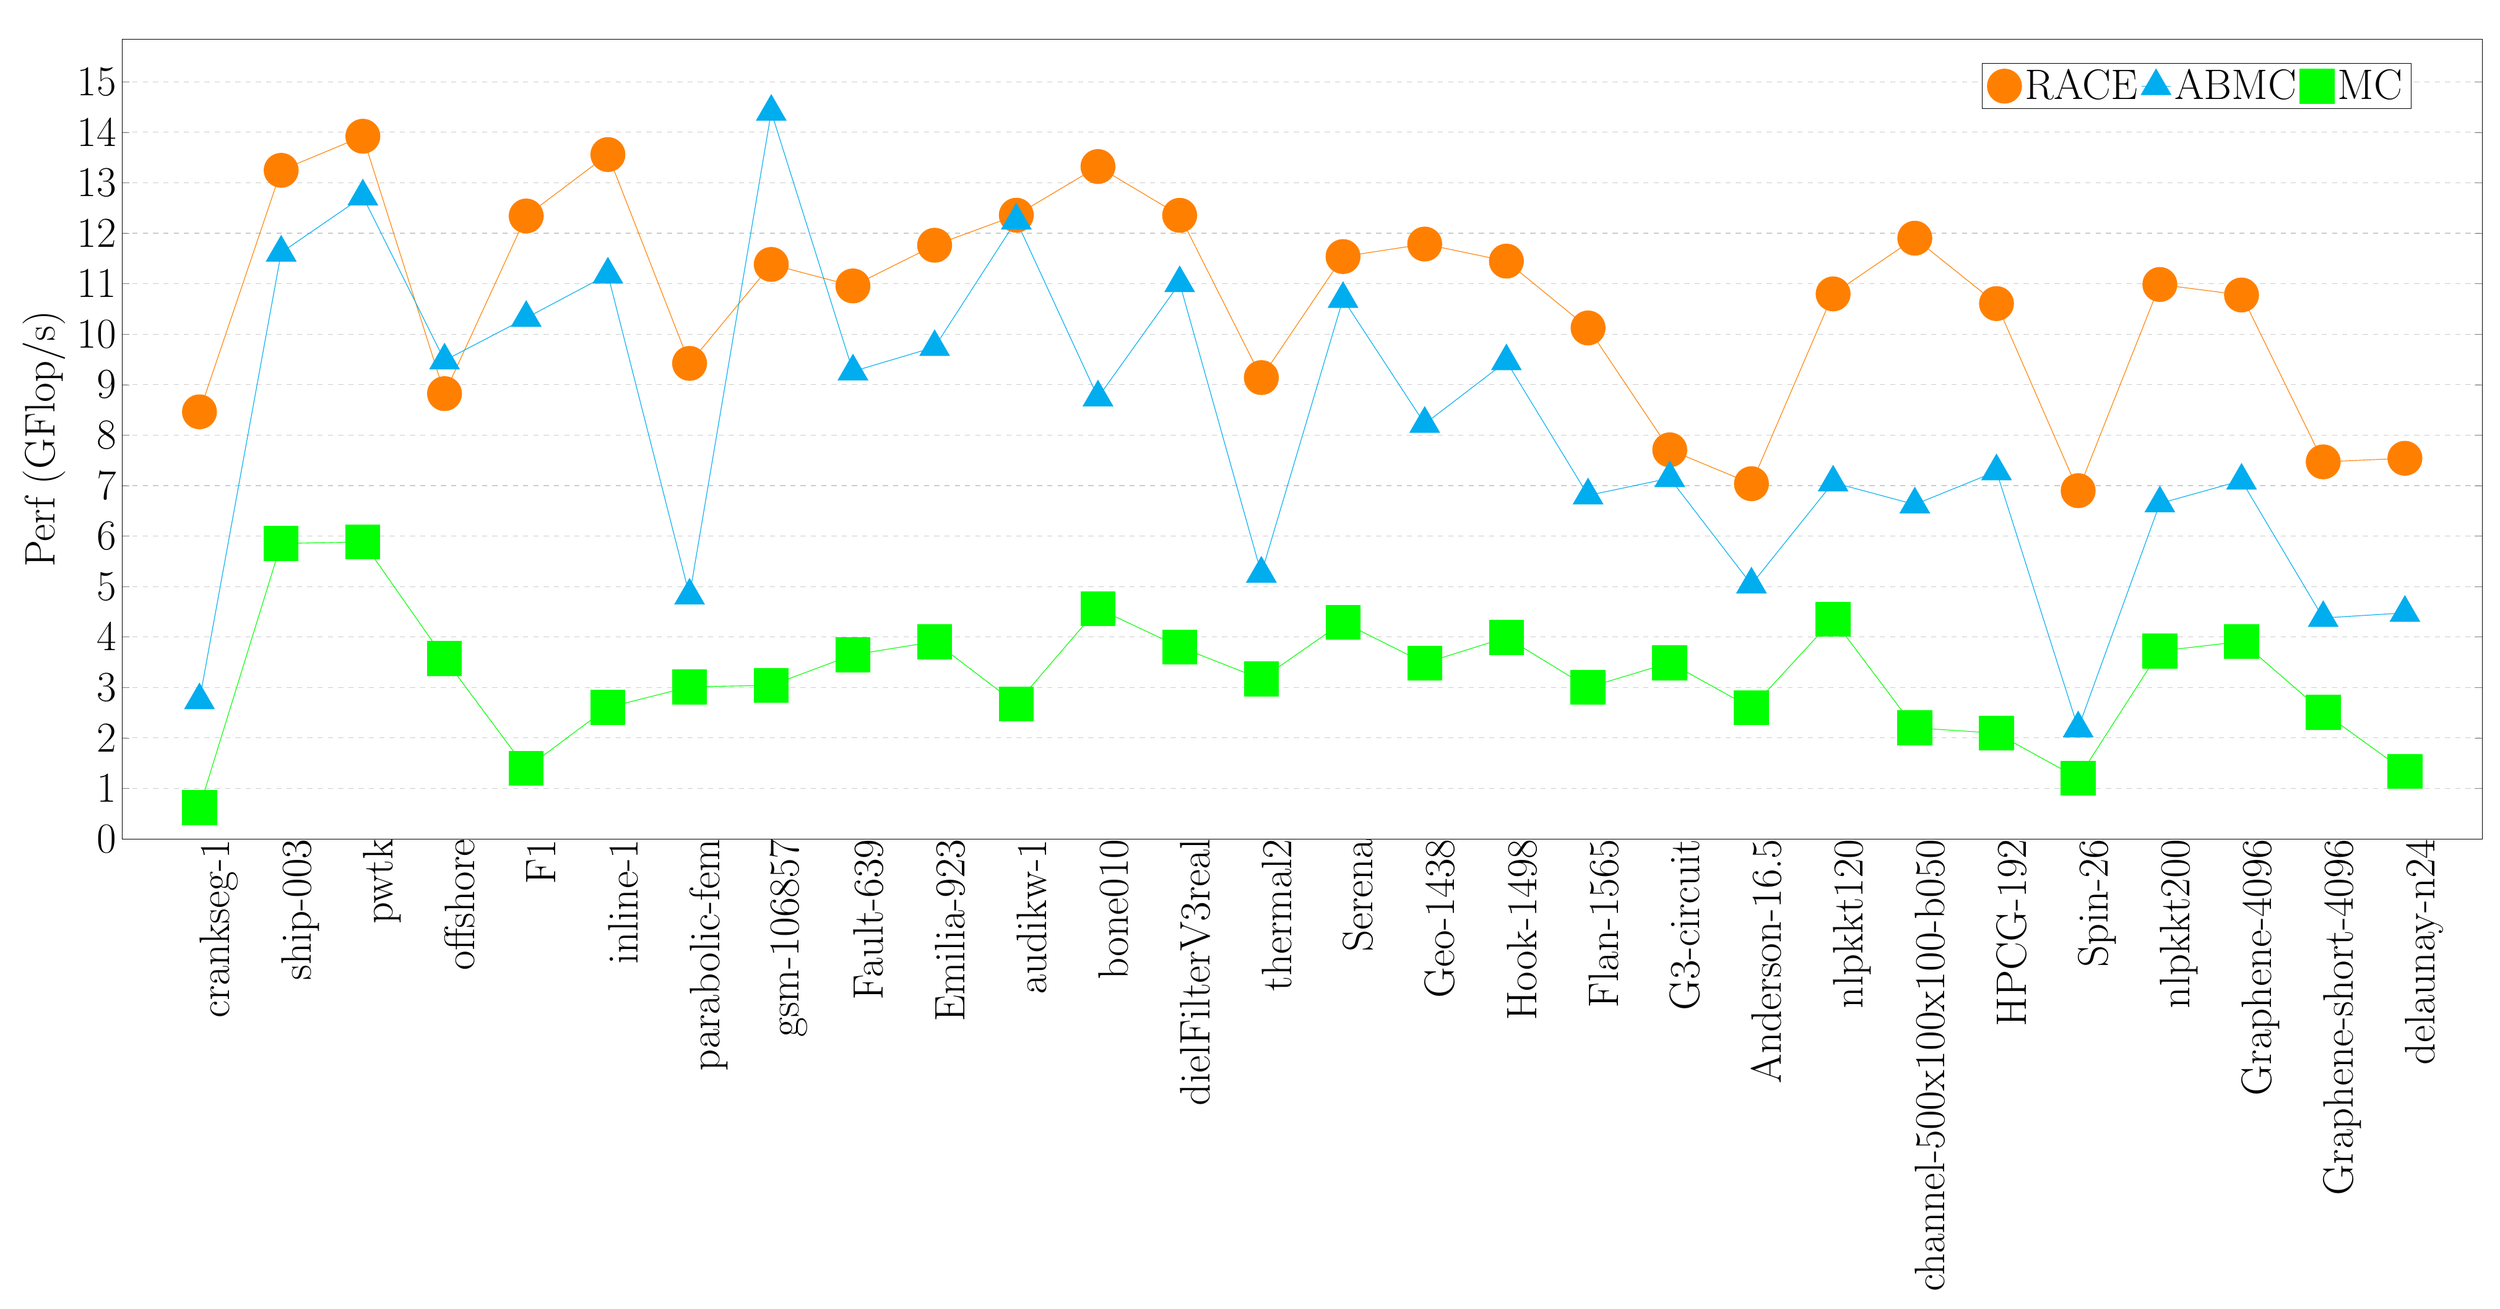
\begin{tikzpicture}
		%	\node at (13.25,15) {\LARGE{}};
			\begin{axis}[
		%	xmin=0.25, xmax=7.25,
			ymin=0, %ymax=3.25,
			xtick={1, 2, 3, 4, 5, 6, 7, 8, 9, 10, 11, 12, 13, 14, 15, 16, 17, 18, 19, 20, 21, 22, 23, 24, 25, 26, 27, 28},
		%	ytick={0,0.5,1,1.5,2,2.5,3},
			xticklabels={crankseg-1, ship-003, pwtk, offshore, F1, inline-1, parabolic-fem, gsm-106857, Fault-639, Emilia-923, audikw-1, bone010, dielFilterV3real, thermal2, Serena, Geo-1438, Hook-1498, Flan-1565, G3-circuit, Anderson-16.5, nlpkkt120, channel-500x100x100-b050, HPCG-192, Spin-26, nlpkkt200, Graphene-4096, Graphene-short-4096, delaunay-n24},
			width  = 50cm,
			height = 18cm,
			major x tick style = transparent,
			%	minor ytick={1, 5, 10, 15, 20, 25, 30 ,35,40},
			grid = minor,	
			%add_bar_commands
			ymajorgrids = true,
			grid style={dashed, gray!40},
			ylabel = {\Huge{Perf (GFlop/s)}},
		%	symbolic x coords={Graphene-2048-2048, Graphene-4096-4096, Spin-24-24-24},
			x tick label style={rotate=90, anchor=north east, inner sep=0mm, font={\Huge}},
			tick label style={font={\Huge}},
			scaled y ticks = false,
			enlarge x limits=0.035,
			legend cell align=left,
			legend style={font=\Huge},
			legend columns=-1,
			legend style={
				%at={(1,1.05)},
				%anchor=south east,
				%column sep=1ex,
				legend pos=north east
			},
			%spl_legend_code
			title= {\Huge\scalebox{1.5}{{}}}
			]

\addplot[mark=*, mark size=10pt, mark options={orange}, draw=orange , y filter/.code={\pgfmathparse{\pgfmathresult*1000}\pgfmathresult}] plot coordinates{(1,.00846153173076923076) (2,.01324681470588235294) (3,.01392203725490196078) (4,.00882238543689320388) (5,.01234152574257425742) (6,.01355900900000000000) (7,.00942133689320388349) (8,.01138242400000000000) (9,.01095599908256880733) (10,.01176216542056074766) (11,.01235745643564356435) (12,.01332161089108910891) (13,.01235514257425742574) (14,.00913995148514851485) (15,.01153803636363636363) (16,.01178579117647058823) (17,.01144760194174757281) (18,.01012329097744360902) (19,.00770854563106796116) (20,.00703714324324324324) (21,.01079820000000000000) (22,.01190178823529411764) (23,.01060615727272727272) (24,.00689933064516129032) (25,.01098451666666666666) (26,.01077660594059405940) (27,.00747042970297029702) (28,.00754096078431372549)};
\addplot[mark=triangle*, mark size=10pt, mark options={cyan}, draw=cyan , y filter/.code={\pgfmathparse{\pgfmathresult*1000}\pgfmathresult}] plot coordinates{(1,.00274606933333333333) (2,.01161557254901960784) (3,.01272802075471698113) (4,.00947787191011235955) (5,.01032287327586206896) (6,.01118077818181818181) (7,.00482023351063829787) (8,.01440536547619047619) (9,.00926169312977099236) (10,.00974393109243697478) (11,.01225110000000000000) (12,.00874625912408759124) (13,.01100942596153846153) (14,.00525437852348993288) (15,.01069810198019801980) (16,.00822354924242424242) (17,.00946195964912280701) (18,.00680515838150289017) (19,.00714632857142857142) (20,.00504018611111111111) (21,.00705996071428571428) (22,.00662585486725663716) (23,.00728254649122807017) (24,.00218936637168141592) (25,.00664720964912280701) (26,.00709740260869565217) (27,.00437658761904761904) (28,.00447836904761904761)};
\addplot[mark=square*, mark size=10pt, mark options={green}, draw=green , y filter/.code={\pgfmathparse{\pgfmathresult*1000}\pgfmathresult}] plot coordinates{(1,.00062049233333333333) (2,.00585221359223300970) (3,.00588453166666666666) (4,.00357235172413793103) (5,.00139696343283582089) (6,.00260585407407407407) (7,.00301229644670050761) (8,.00304297926829268292) (9,.00364767843137254901) (10,.00390729727891156462) (11,.00267594537815126050) (12,.00456334028776978417) (13,.00380282407407407407) (14,.00316779933774834437) (15,.00429262689075630252) (16,.00348306535947712418) (17,.00399057686567164179) (18,.00300092588832487309) (19,.00348970655737704918) (20,.00259613511450381679) (21,.00435293902439024390) (22,.00220035500000000000) (23,.00209408897058823529) (24,.00120325038759689922) (25,.00372281129032258064) (26,.00391036771653543307) (27,.00250906140350877192) (28,.00133974041095890410)};
	%addplot cmd

	\legend{RACE, ABMC, MC}

	\end{axis}			
\end{tikzpicture}

\end{document}

